\documentclass[12pt,fleqn]{article}
\setlength{\parindent}{0pt}
\usepackage{graphicx}
\usepackage{listings}
\usepackage[latin5]{inputenc}
\setlength{\parskip}{8pt}
\setlength{\parsep}{0pt}
\setlength{\headsep}{0pt}
\setlength{\topskip}{0pt}
\setlength{\topmargin}{0pt}
\setlength{\topsep}{0pt}
\setlength{\partopsep}{0pt}
\setlength{\mathindent}{0cm}

\begin{document}
MIT OCW Cok Degiskenli Calculus - Ders 10

Bugunku konumuz kritik noktalarin minima mi, maksima mi, yoksa eger noktasi
mi oldugunu anlama teknikleri. Kritik noktalar kismi turevlerin hepsinin
sifir oldugu noktadir, mesela 2 degiskenli fonksiyon icin $f_x=0$, $f_y=0$
olmalidir. 

3 degisik kritik nokta cesidi gorduk, lokal minima, lokal maksima, ve
eger (saddle) noktalari. 

Bir fonksiyonun birden fazla kritik noktasi olabilir. Mesela soyle bir
fonksiyon

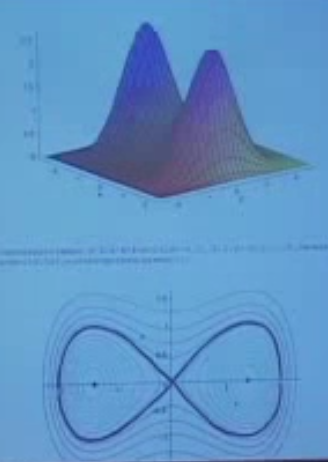
\includegraphics[height=4cm]{10_1.png}















\end{document}
